%--- iliad -------------------------------------------------------------------
% title: "Instrumental Convergence"
% summary: >-
%   We discuss a simple mathematical formalization of what it means to "seek
%   power" in a Markov decision process (MDP), and conditions under which such
%   behavior emerges.
% contributors:
%   - "Leon Lang (ILIAD), based on work by Alex Turner et al."
% slides: https://drive.google.com/drive/folders/127bVYqhJPhzA7S71FwTqeyNKKKkjM2NB
%--- end ----------------------------------------------------------------------
\documentclass[11pt]{article}
\IfFileExists{iliad.sty}{\usepackage[boxes]{iliad}}{\usepackage[boxes]{../iliad}}

% ---- Free zone -------------------------------------------------------------
\usepackage[T1]{fontenc}                    % Ćirković
\usepackage{mathtools}                      % \coloneqq
\usepackage{tikz}
\usetikzlibrary{positioning, arrows.meta}

% Math macros, verbatim from the source sheet.
\newcommand{\cS}{\mathcal{S}}
\newcommand{\cA}{\mathcal{A}}
\newcommand{\R}{\mathbb{R}}
\newcommand{\E}{\mathbb{E}}
\newcommand{\Prob}{\mathbb{P}}
\newcommand{\Dist}{\mathcal{D}}    % a distribution over reward functions
\newcommand{\F}{\mathcal{F}}       % option set: visitation distributions reachable from a state
\newcommand{\mset}[1]{\{\!\{\,#1\,\}\!\}}   % multiset (unordered, with multiplicity)

\title{Instrumental Convergence}
\author{\authorname{Leon Lang}\\ \affiliation{ILIAD}}
\date{April 2026}

\begin{document}
\maketitle

% Module Intent and Prerequisites, from the day's Google-Doc tab. They describe
% the day rather than the sheet, and moved here when the sheet became D.6.1.
\begin{learningoutcomes}
The students understand the proofs for power-seeking tendencies based on Alex
Turner's work, and can critically examine the weaknesses and implications of
this work. This work is important since power-seeking behavior is one of the
most severe risks that AI may pose, and this may be the most rigorous work to
date establishing it under clear assumptions and definitions. The goals are
achieved through an initial presentation, by working through an exercise sheet,
and by reading and discussing the original papers.
\end{learningoutcomes}

\paragraph{Prerequisites.}

A basic familiarity with reinforcement learning is sufficient.

\paragraph{Roadmap for today.}

Outline of the day:

\begin{itemize}
  \item 10:00 -- 11:00: Presentation
  \item 11:15 -- 13:15: Solving of exercises
  \item 14:15 -- 15:15: Solving more exercises
  \item 15:30 -- 16:15: Reading
\begin{itemize}
  \item One of the three main papers is read by everyone.
\end{itemize}
  \item 16:15 -- 16:45: Discussion
\begin{itemize}
  \item Participants who read different papers discuss together.
\end{itemize}
  \item 17:00 -- 17:15: Brainstorming of limitations / critiques / ideas and theoretical/empirical hypotheses
  \item 17:15 -- 17:45: Students present and discuss their ideas
\end{itemize}

% The day's teacher-facing sections, from its Google-Doc tab, in the tab's own
% order: "Intents of subsection" and "Teaching notes" sit after the timetable.
% Collapsed on the web, so they stay out of the student's reading flow.
\begin{teachingnote}[Intents of subsection]
In the exercises, the participants learn to understand one model of the reward
function distribution, decision rule, and conceptualization of ``power'' in
detail, and learn the mathematical arguments connecting them in detail. This is
useful as learning one model in detail helps to quickly understand all variations
that are discussed in many of Turner's papers.

The readings teach the participants variations of the concepts and results, which
may help them to appreciate the breadth and limitations of the results better.

Finally, the brainstorming of limitations and ideas gets participants into a
critical mindset and makes them think through whether the theoretical notions of
power capture what we mean, and how to go beyond. This is important since the
applicability of the results to actual AI training processes is questioned by
many people in the community.
\end{teachingnote}

\begin{teachingnote}[Teaching notes]
I think the setup I chose (together with Claude) in the exercise sheet has some
advantages compared to Turner's original treatment of the results:

\begin{itemize}
  \item The use of an invariant measure avoids ``orbit counting'' and grounds everything in the more justified notion of probabilities of various outcomes.
  \item We work with \emph{a subgroup} of the symmetric group, and thus avoid the unjustified assumption that the measure on reward functions is invariant under arbitrary symmetries (which it obviously isn't!)
  \item The notion of a dynamics embedding grounds the notion of ``more options'' into actual MDP dynamics.
  \item The use of score functions allows us to achieve a power-seeking result for one-sided dynamics embeddings and under non-trivial discount factors.
\end{itemize}

Overall, I think this makes the results much more interpretable, and I would thus
not recommend to go back to the framing of any of Turner's particular papers.
\end{teachingnote}

\section*{Introduction}


Suppose we build an AI and give it a goal.
A long-standing worry --- \emph{instrumental convergence} --- holds that for a very wide
range of encoded objectives, a sufficiently capable agent converges on the same handful
of intermediate strategies, because they are useful almost regardless of the final goal:
acquire resources, stay operational, and keep one's options open
\cite{omohundro2008basic,bostrom2014superintelligence}. We call the drive towards
them \textbf{seeking power}, where ``power'' means \emph{the ability to achieve a wide
range of goals} --- being in a position from which many futures remain reachable.

This worksheet attempts to model such claims mathematically and establish proofs for them. We study the following question.

\begin{callout}
\textbf{The question.}
We train an AI in some environment (a Markov decision process) to perform well according
to a reward function. \textbf{Will it seek power, or not?}
\end{callout}

The central claim we will
build up to is the following.

\begin{quote}
\emph{Under many suitable decision rules for how to act, and for the majority of reward
functions, keeping more options open is the likelier outcome than keeping fewer options
open.}
\end{quote}

``Keeping more options open'' is then the operationalization for ``seeking power'', which can also be shown to connect to the ability to achieve a wide variety of goals.
This is a statement about a \emph{tendency}, not about \emph{every} goal. The results we prove are the core cases from
\cite{turner2021optimal,turner2022parametrically}, with an application to
\emph{trained} agents in \cite{krakovna2023power} and a measure-theoretic re-examination
of ``most goals'' in \cite{jacek2023categorical}. These works provide many generalizations of the claims in this worksheet.

Making the central claim precise requires formalising three phrases. The rest of the
worksheet is organised around them and then proving the result:

\begin{enumerate}
  \item \emph{for the majority of reward functions}: How do we count reward functions?
  \item \emph{a suitable decision rule}: Which ways of turning a
  reward function into behaviour are covered (maximization is only one)?
  \item \emph{keeping more options open}: How do we measure that one situation leaves more achievable than
  another?
\end{enumerate}

We formalise all three and then prove the resulting theorems. The setup below fixes the
environment; the three numbered sections that follow take up points~(1), (2), and~(3) in turn.

% ================================================


\section*{Setup}

Throughout the worksheet we fix a discount factor $\gamma \in (0,1)$ once and for all.

\subsection*{The environment}

We separate the \emph{environment} (its states and dynamics) from the \emph{goal} (a
reward function) since we want to make claims about the whole set of reward functions.

\begin{definition}[Rewardless MDP]\label{def:mdp}
A \textbf{rewardless Markov decision process (MDP)} is a tuple
$\langle \cS, \cA, T\rangle$ consisting of
\begin{itemize}\itemsep=2pt
  \item a finite \textbf{state space} $\cS$, with $d := |\cS|$ states;
  \item a finite \textbf{action space} $\cA$;
  \item a \textbf{transition function} $T : \cS \times \cA \to \Delta\cS$, where
  $\Delta X$ denotes the set of probability distributions over a finite set $X$. Taking
  action $a$ in state $s$ moves the agent to state $s'$ with probability
  $T(s' \mid s, a)$.
\end{itemize}
A \textbf{policy} $\pi : \cS \to \cA$ specifies which action the agent takes in each
state.\footnote{We restrict to deterministic policies since many of our analyses expect a finite set of policies.} We write
$e_s \in \R^{d}$ for the indicator vector of state $s$.
\end{definition}


\begin{definition}[Reward function]\label{def:reward}
A \textbf{reward function} assigns a real number $r(s)$ to each state $s\in\cS$. Since
$\cS$ has $d$ elements, a reward function is simply a vector
$$
r \;\in\; \R^{d},
$$
so we take the \textbf{space of goals to be all of $\R^d$}. 
\end{definition}


\section{For the majority of reward functions}

We cannot expect a power-seeking conclusion for \emph{every} reward function: a goal that
intrinsically rewards a single shutdown state will send the agent straight there.
So what are the reward functions we should expect in reality and how likely are they to incentivize power-seeking behavior?

Ideally, we would train our AI on ``the'' ``correct'' reward function: one that
integrates the wellbeing, ethics, and preferences of everyone affected, similar to a constitution. In practice we never hold such a reward function in our hands,
for at least two reasons.
\begin{itemize}\itemsep=2pt
  \item \textbf{The specification is moving.} The written rules, norms, and intentions we
  want to distill into a reward function change over time and between the humans involved in their specification.
  \item \textbf{The learned reward is procedure-dependent.} The techniques that turn rules
  into an actual reward signal (human feedback, preference models, fine-tuning) depend
  heavily on the training method and setup and perhaps even random seeds, so the same intent yields different reward
  functions under different procedures.
\end{itemize}

Thus, let's fix a distribution (Borel measure) over reward functions that captures our uncertainty over what emerges in realistic specification procedures:
$$
\Dist \;\in\; \Delta(\R^{d}), \qquad d = |\cS|,
$$
and read ``power-seeking holds for $\Dist$-most reward functions'' as a statement about
$r \sim \Dist$.
Note that $\Dist$ may have \emph{restricted support}, i.e.\ give zero probability to large regions
of $\R^{d}$. This effectively shrinks down the goal set.

\subsection*{Symmetries of the reward distribution}

Often $\Dist$ carries structure of its own. Two regions of the state space may look alike to the
specification procedure, so the
procedure is no more likely to attach a given reward to one than to the other. The relabelling of
states that swaps such regions then leaves $\Dist$ unchanged.

\begin{definition}[Symmetry of $\Dist$]\label{def:D_symmetry}
A permutation $\phi$ of the states $\cS$ \textbf{relabels} a reward function $r$ into $\phi\cdot r$,
where $(\phi\cdot r)(s) := r(\phi^{-1}(s))$. We call $\phi$ a \textbf{symmetry of $\Dist$} if $\phi_*\Dist = \Dist$, i.e.\
$\Dist(\phi^{-1}E) = \Dist(E)$ for every Borel $E\subseteq\R^d$. The symmetries of $\Dist$ form a
group, assumed nontrivial throughout.
\end{definition}

As a trivial example, if the per-state rewards are independent and identically distributed --- say
each $r(s)$ is uniform on $[0,1]$ --- then \emph{every} permutation of states is a symmetry of
$\Dist$. Realistic distributions are far less symmetric; the results ahead need only that
\emph{some} nontrivial symmetry exists.


% ===================================================================

\section{Suitable decision rules}\label{prob:decision_rules}

This section takes up point~(2): \emph{which} ways of turning a reward function into
behaviour we will cover. We first extend the reinforcement-learning setup with the value
function and a change of variables that isolates the role of the reward; we then define
decision rules and single out the class --- the \emph{expected-utility-determined} rules
--- that we treat as ``suitable''.

\subsection*{Value functions and the goal of reinforcement learning}


\begin{definition}[Value function]\label{def:value}
For a policy $\pi$, reward $r\in\R^d$, and start state $s$, the \textbf{value} of $\pi$ is
the expected discounted reward collected from $s$,
$$
V^\pi_r(s) \;:=\; \E_\pi\!\Big[\,\textstyle\sum_{t=0}^{\infty} \gamma^t\, r(s_t)\ \Big|\ s_0 = s\,\Big],
$$
the expectation taken over trajectories $s_0, s_1, s_2, \dots$ generated by $\pi$. The goal of reinforcement learning is to find an \textbf{optimal policy}, i.e.\ attaining the \textbf{optimal value}
$$
V^\ast_r(s) \;:=\; \max_\pi V^\pi_r(s)
$$
simultaneously at every state $s$. For finite MDPs such a policy exists, as we have shown on the RL day.
\end{definition}

\subsection*{Isolating the reward: state-visitation distributions}

In $V^\pi_r(s)$ the reward $r$ enters \emph{linearly}, but the policy $\pi$ enters through
the whole distribution over trajectories. We disentangle the two by packing everything the
policy does into a single vector, after which the value becomes a plain inner product
with~$r$.

\begin{definition}[State-visitation distribution]\label{def:visit}
Let $T^\pi$ be the transition matrix induced by $\pi$, with entry $(T^\pi)_{s',s}$ the
probability of moving to $s'$ from $s$ under $\pi$:
$$T^{\pi}_{s',s} = \sum_{a} T(s' \ | \ s, a) \cdot \pi(a | s) = T(s' \ | \ s, \pi(s)),$$
where we used that our policies are assumed deterministic throughout.
Then $(T^\pi)^t e_s$ is the state
distribution after $t$ steps starting from $s$. The \textbf{(discounted) state-visitation
distribution} of $\pi$ from $s$ is
$$
f^\pi(s) \;:=\; \sum_{t=0}^{\infty} \gamma^t (T^\pi)^t e_s \;=\; (I - \gamma T^\pi)^{-1} e_s \ \in\ \R^d,
$$
whose $s'$-component
$f^\pi(s)_{s'} = \sum_{t=0}^\infty \gamma^t\, \Prob_\pi[s_t = s' \mid s_0 = s]$ is the total
expected discounted time $\pi$ spends in $s'$ when started at $s$.
\end{definition}

\begin{definition}[Options available at a state]\label{def:options}
The \textbf{option set} at $s$ is
$$
\F(s) \;:=\; \bigl\{\, f^\pi(s) \;:\; \pi \text{ a policy}\,\bigr\} \ \subseteq\ \R^d,
$$
the set of all state-visitation distributions the agent can realize from $s$. We call its
elements the \textbf{options} at $s$.
As we assumed all policies to be deterministic, $\F(s)$ is finite for every state $s$.
\end{definition}



\begin{exercise}
\label{prob:value_linear} Show that the value is the inner product of the
visitation distribution with the reward:
\begin{callout}
\textbf{Value is linear in the reward.}
$$
V^\pi_r(s) \;=\; f^\pi(s)^\top r.
$$
\end{callout}
Deduce that finding an optimal policy is a linear optimization over the option set:
$V^\ast_r(s) = \max_{f \in \F(s)} f^\top r$.
\end{exercise}

\begin{solution}[prob:value_linear]
Because $r$ depends only on the state and the trajectory is generated by $\pi$,
\begin{align*}
V^\pi_r(s)
&= \E_\pi\Big[\textstyle\sum_{t=0}^\infty \gamma^t r(s_t)\ \Big|\ s_0 = s\Big]
 = \sum_{t=0}^\infty \gamma^t\, \E_\pi\bigl[r(s_t)\mid s_0 = s\bigr] \\
&= \sum_{t=0}^\infty \gamma^t \sum_{s'\in\cS} \Prob_\pi[s_t = s' \mid s_0 = s]\, r(s') \\
&= \sum_{s'\in\cS} \underbrace{\Big(\sum_{t=0}^\infty \gamma^t\, \Prob_\pi[s_t = s'\mid s_0=s]\Big)}_{=\ f^\pi(s)_{s'}} r(s') \\
&= f^\pi(s)^\top r.
\end{align*}
Taking the maximum over policies,
$$
V^\ast_r(s) = \max_\pi V^\pi_r(s) = \max_\pi f^\pi(s)^\top r = \max_{f \in \F(s)} f^\top r,
$$
a linear objective maximized over the option set $\F(s)$.
\end{solution}

The identity $V^\pi_r(s) = f^\pi(s)^\top r$ effectively linearizes the problem: it turns
``act well under $r$'' into ``pick a high-quality option from $\F(s)$'', with the reward
appearing only through the inner product. 

\subsection*{Decision rules}

A decision rule describes the selection of an option from $\F(s)$ given a reward function, with potential randomness in the selection procedure. 

\begin{definition}[Decision rule]\label{def:decision_rule}
A \textbf{decision rule} assigns, to each state $s$ and reward $r \in \R^d$, a probability
distribution $p(\cdot \mid s, r)$ over the accessible options $\F(s)$: for each subset
$X \subseteq \F(s)$,
$$
p(X \mid s, r) \in [0,1]
$$
is the probability that the agent's selected option lies in $X$ (options outside $\F(s)$
receive zero probability by construction). The \textbf{quality} of an option $f \in \F(s)$
under $r$ is its value $f^\top r$ (\cref{prob:value_linear}).
\end{definition}

\begin{definition}[Expected-utility-determined rule]\label{def:eu_determined}
For a finite set $Y \subseteq \R^d$ of options, write
$$
\mathrm{EU}_r(Y) \;:=\; \mset{\, f^\top r : f \in Y \,}
$$
for the \textbf{multiset} of qualities of $Y$ under $r$ --- the values $f^\top r$ for
$f \in Y$, counted with multiplicity but carrying \emph{no order}. A decision rule is
\textbf{expected-utility-determined} (EU-determined) if there is a single function $g$,
\emph{defined on multisets}, such that for every state $s$, reward $r \in \R^d$, and
$X \subseteq \F(s)$,
$$
p(X \mid s, r) \;=\; g\bigl(\mathrm{EU}_r(X),\, \mathrm{EU}_r(\F(s))\bigr).
$$
Because $g$ takes \emph{multisets} as inputs, it cannot depend on any ordering of the
options --- only on which qualities occur and with what multiplicity. Thus $p$ sees the
options only through the two multisets of qualities, those of the chosen set $X$ and of the
full menu $\F(s)$. These are the rules we call \textbf{suitable} in point~(2) of the
introduction.
\end{definition}

The basic example is exact optimization, with ties broken uniformly; but noisy and
threshold-based rules qualify just as well. We record three options here, but there are many others.

\begin{definition}[Three EU-determined decision rules]\label{def:rules}
Fix a state $s$ and a reward $r$, and write $M(r) := \max_{f \in \F(s)} f^\top r$ for the
maximal quality.  For $X \subseteq \F(s)$:
\begin{itemize}\itemsep=5pt
  \item \textbf{Uniform tie-breaking} (optimal choice with ties split evenly): Choose uniformly among all maximizers,
  $$
  \mathrm{FracOpt}(X \mid s, r) \;:=\;
  \frac{\bigl|\{\, f \in X : f^\top r = M(r) \,\}\bigr|}{\bigl|\{\, f \in \F(s) : f^\top r = M(r) \,\}\bigr|}.
  $$
  \item \textbf{Boltzmann rational} (softmax) at temperature $T > 0$: weight options by the
  exponential of their quality,
  $$
  \mathrm{Bz}_T(X \mid s, r) \;:=\;
  \frac{\sum_{f \in X} e^{\,f^\top r / T}}{\sum_{f \in \F(s)} e^{\,f^\top r / T}}.
  $$
  \item \textbf{Satisficing} at threshold $t \in \R$: pick uniformly among the options that
  are ``good enough'',
  $$
  \mathrm{Sat}_t(X \mid s, r) \;:=\; \frac{\bigl|X \cap \F_{\ge t}(s)\bigr|}{\bigl|\F_{\ge t}(s)\bigr|},
  \qquad \F_{\ge t}(s) := \{\, f \in \F(s) : f^\top r \ge t \,\}.
  $$
  This is only defined if $\F_{\ge t}(s) \neq \emptyset$.
\end{itemize}
\end{definition}

\begin{exercise}
\label{prob:rules_eu} Verify that $\mathrm{FracOpt}$, $\mathrm{Bz}_T$, and
$\mathrm{Sat}_t$ are each EU-determined.
\end{exercise}

\begin{solution}[prob:rules_eu]
Each rule is, by inspection, a function of the two quality-multisets $\mathrm{EU}_r(X)$ and
$\mathrm{EU}_r(\F(s))$ alone --- that is, of the form
$g\bigl(\mathrm{EU}_r(X), \mathrm{EU}_r(\F(s))\bigr)$:
\begin{itemize}\itemsep=2pt
  \item $\mathrm{FracOpt}$: with $M(r) = \max \mathrm{EU}_r(\F(s))$, it is the multiplicity of
  $M(r)$ in $\mathrm{EU}_r(X)$ divided by its multiplicity in $\mathrm{EU}_r(\F(s))$.
  \item $\mathrm{Bz}_T$: it is $\sum_{u \in \mathrm{EU}_r(X)} e^{u/T}$ divided by
  $\sum_{u \in \mathrm{EU}_r(\F(s))} e^{u/T}$ (note these sums take into account the multiplicity of $u$ in the respective multisets).
  \item $\mathrm{Sat}_t$: it is the number of entries $\ge t$ in $\mathrm{EU}_r(X)$ divided by
  the number of entries $\ge t$ in $\mathrm{EU}_r(\F(s))$.
\end{itemize}
None refers to an option $f$ except through its quality $f^\top r$, so each is EU-determined.
\end{solution}

A further family will carry the main result: rules that weight each option by a fixed transform of
its quality and normalize.

\begin{definition}[Score rule]\label{def:score_rule}
A decision rule $p$ is a \textbf{score rule} if there is a nondecreasing
$\nu : \R \to [0,\infty)$ with
$$
p(\{f\}\mid s, r) \;=\; \frac{\nu(f^\top r)}{\sum_{h\in\F(s)}\nu(h^\top r)} \qquad (f \in \F(s)),
$$
so that $p(X\mid s,r) = \sum_{f\in X}\nu(f^\top r)\big/\sum_{h\in\F(s)}\nu(h^\top r)$ (defined when
the normalizer is positive). Both $\mathrm{Bz}_T$ (with $\nu(q) = e^{q/T}$) and $\mathrm{Sat}_t$
(with $\nu(q) = \mathbf{1}[q\ge t]$) are score rules. ($\mathrm{FracOpt}$ is \emph{not} a score
rule: its cutoff is not fixed.)
\end{definition}

\subsection*{Relabelling states}

In \cref{def:D_symmetry} a permutation relabelled a reward function; the same relabelling acts on
options too. We record the action and the one property of it we will need later: it preserves
quality.

\begin{definition}[Permutation action]\label{def:perm_action}
A permutation $\phi$ of the state set $\cS$ acts on $\R^d \cong \R^{\cS}$ by permuting
coordinates: it sends $x \in \R^d$ to the vector $\phi \cdot x$ with
$$(\phi \cdot x)_{s} \coloneqq x_{\phi^{-1}(s)}$$
and a set of options $X$ to
$$\phi \cdot X \coloneqq \{\, \phi \cdot f : f \in X \,\}.$$
\end{definition}

\begin{exercise}
\label{prob:quality_invariant} Show that the permutation action preserves
inner products: for every permutation $\phi$ and all $x, y \in \R^d$,
$$
(\phi \cdot x)^\top (\phi \cdot y) = x^\top y .
$$
In particular, relabelling a reward and an option together leaves the quality unchanged:
$(\phi \cdot f)^\top (\phi \cdot r) = f^\top r$.
\end{exercise}

\begin{solution}[prob:quality_invariant]
Writing out the inner product and reindexing the sum by $s' = \phi^{-1}(s)$ (a bijection
of $\cS$):
$$
(\phi \cdot x)^\top (\phi \cdot y)
= \sum_{s \in \cS} (\phi \cdot x)_{s}\, (\phi \cdot y)_{s}
= \sum_{s \in \cS} x_{\phi^{-1}(s)}\, y_{\phi^{-1}(s)}
= \sum_{s' \in \cS} x_{s'}\, y_{s'}
= x^\top y .
$$
\end{solution}

% ===================================================================

\section{Keeping options open}\label{prob:options}

We now take up point~(3): what it means for one action to keep more options open than another.
The options realizable from $s$ decompose according to the first action taken.

\begin{definition}[Options under an action]\label{def:options_action}
For an action $a$ at $s$, the \textbf{options under $a$} are the visitation distributions
realizable from $s$ when the first action is $a$:
$$
\F(s \mid a) \;:=\; \bigl\{\, f^\pi(s) : \pi \text{ a policy with } \pi(s) = a \,\bigr\} \ \subseteq\ \F(s).
$$
\end{definition}

The right comparison is \emph{containment up to relabelling}: $a$ is at least as rich as $a'$
when every option available after $a'$ has a relabelled twin available after $a$.

\begin{definition}[Keeping at least as many options open]\label{def:keep_options}
$\F(s\mid a)$ \textbf{contains a copy of} $\F(s\mid a')$ if $\phi \cdot \F(s\mid a') \subseteq \F(s\mid a)$
for some permutation $\phi$ of $\cS$. When this holds we say \textbf{$a$ keeps at least as many
options open as $a'$ at $s$}.
\end{definition}


The containment quantifies over all policies, so it is awkward to check directly. It follows from a
\emph{one-sided} structural condition on the dynamics: $\phi$ need only embed the part of the
environment reachable after $a'$ into the part reachable after $a$, and may leave the $a$-branch
with extra room.

\begin{definition}[One-sided dynamics embedding]\label{def:dyn_embedding}
Let $R'$ be the set of states reachable from $s$ along a trajectory whose first action is $a'$
(so $s \in R'$). A permutation $\phi$ of $\cS$ with $\phi(s) = s$ \textbf{embeds $a'$ into $a$
at $s$} if
\begin{enumerate}
  \item $T(\phi(s'') \mid s, a) = T(s'' \mid s, a')$ for all $s''$; and
  \item for every $s' \in R'$ with $s' \ne s$ and every action $b$, there is an action
  $b'$ with $T(\phi(s'') \mid \phi(s'), b') = T(s'' \mid s', b)$ for all $s''$.
\end{enumerate}
\end{definition}

\begin{exercise}
\label{prob:embedding_gives_copy} Show that if $\phi$ embeds $a'$ into $a$ at
$s$, then $\phi \cdot \F(s\mid a') \subseteq \F(s\mid a)$ --- so $a$ keeps at least as many
options open as $a'$ at $s$.
\end{exercise}
\begin{hint}
given a policy $\pi$ with $\pi(s)=a'$, relabel it into a policy $\rho$ with
$\rho(s)=a$ and $f^\rho(s) = \phi \cdot f^\pi(s)$.
\end{hint}

\begin{solution}[prob:embedding_gives_copy]
We use two facts: the $s'$-th column of the transition matrix is the one-step law
$T^\pi e_{s'} = T(\cdot\mid s',\pi(s'))$ (with $T^\pi$ linear), and relabelling sends indicators to
indicators, $\phi\cdot e_{s'} = e_{\phi(s')}$ (with $\phi\cdot$ linear).

Fix a policy $\pi$ with $\pi(s) = a'$, and define a policy $\rho$ by $\rho(s) := a$ and, for
each $s' \in R'$ with $s' \ne s$, $\rho(\phi(s')) := b'$, the action supplied by (ii) for
$b = \pi(s')$ (arbitrary off $\phi(R')$; $\phi$ is injective, so this is unambiguous).

\emph{The $a'$-dynamics stay in $R'$.} If $v$ is supported on $R'$, so is $T^\pi v$: from any
$s' \in R'$ the $\pi$-successors are again reachable from $s$ via $a'$, hence lie in $R'$. In
particular $(T^\pi)^t e_s$ is supported on $R'$ for every $t$.

\emph{Intertwining on $R'$.} For every $s' \in R'$,
\begin{equation*}
T^\rho e_{\phi(s')} = T(\cdot \mid \phi(s'),\, \rho(\phi(s'))) = \phi \cdot T(\cdot\mid s',\, \pi(s')) = \phi\cdot(T^\pi e_{s'}),
\end{equation*}
where for $s' = s$ this is (i) (using $\pi(s)=a'$ and $\rho(s)=a$), and for $s' \ne s$ it is
(ii) (with $b = \pi(s')$). Hence, for $v$ supported on $R'$,
$$
T^\rho(\phi\cdot v) = \sum_{s'\in R'} v_{s'}\, T^\rho e_{\phi(s')} = \sum_{s'\in R'} v_{s'}\, \phi\cdot(T^\pi e_{s'}) = \phi\cdot(T^\pi v).
$$

\emph{Iterating.} By induction $(T^\rho)^t e_s = \phi\cdot(T^\pi)^t e_s$ for
every $t$: the base case is $\phi\cdot e_s = e_{\phi(s)} = e_s$, and the step applies the
intertwining to $v = (T^\pi)^t e_s$, which is supported on $R'$. Summing the discounted series,
$f^\rho(s) = \phi\cdot f^\pi(s)$. Since $\rho(s) = a$, we have $f^\rho(s) \in \F(s\mid a)$, so
$\phi\cdot f^\pi(s) \in \F(s\mid a)$; as $\pi$ ranged over all policies with $\pi(s)=a'$, this
gives $\phi\cdot\F(s\mid a') \subseteq \F(s\mid a)$.
\end{solution}

\section*{The result}

The three ingredients now combine: a suitable rule (a score rule, \cref{def:score_rule}), an action
that keeps more options open (an embedding $\phi$, \cref{def:keep_options}), and a symmetric reward
distribution ($\phi$ a symmetry of $\Dist$, \cref{def:D_symmetry}). Fix $s$ and actions $a,a'$, and
abbreviate the probabilities that the rule $p$ lands its choice in the $a$- and $a'$-options:
$$
A(r) := p\bigl(\F(s\mid a)\mid s,r\bigr), \qquad A'(r) := p\bigl(\F(s\mid a')\mid s,r\bigr).
$$


\begin{exercise}
\label{prob:power_seeking} Let $p$ be a score rule, and let $\phi$ be an
involution that
\begin{itemize}\itemsep=2pt
  \item[1.] embeds $a'$ into $a$: $\ \phi\cdot\F(s\mid a') \subseteq \F(s\mid a)$; and
  \item[2.] is a symmetry of $\Dist$: $\ \phi_*\Dist = \Dist$.
\end{itemize}
Show that

\begin{callout}
\textbf{Keeping options open is favoured.}
$$
\Prob_{r\sim\Dist}\bigl[\, A(r) \ge A'(r) \,\bigr] \;\ge\; \tfrac{1}{2}.
$$
\end{callout}

\noindent That is: for $\Dist$-most reward functions, $p$ is at least as likely to act through the
option-richer action $a$ as through $a'$.
\end{exercise}
\begin{hint}
write $N_r(X) := \sum_{f\in X}\nu(f^\top r)$, so $A = N_r(\F(s\mid a))/N_r(\F(s))$ and
likewise $A'$. From \cref{prob:quality_invariant}, $N_{\phi\cdot r}(\phi\cdot Y) = N_r(Y)$ for every
$Y$. Compare $A, A'$ at $r$ and at $\phi\cdot r$; the denominators cancel.
\end{hint}

\begin{solution}[prob:power_seeking]
Write $N_r(X) = \sum_{f\in X}\nu(f^\top r)$, so $p(X\mid s,r) = N_r(X)/N_r(\F(s))$, and put
$G := \phi\cdot\F(s\mid a') \subseteq \F(s\mid a)$ --- a copy of $\F(s\mid a')$ inside $\F(s\mid a)$,
as $\phi$ is injective. Termwise, \cref{prob:quality_invariant} gives the \textbf{swap identity}
$$
N_{\phi\cdot r}(\phi\cdot Y) = \sum_{f\in Y}\nu\bigl((\phi\cdot f)^\top(\phi\cdot r)\bigr) = \sum_{f\in Y}\nu(f^\top r) = N_r(Y).
$$

\emph{Retargeting.} Suppose $A'(r) > A(r)$. These share the denominator $N_r(\F(s))$, so
$N_r(\F(s\mid a')) > N_r(\F(s\mid a)) \ge N_r(G)$ --- the last step since $G\subseteq\F(s\mid a)$ and
$\nu\ge0$. Evaluate at $\phi\cdot r$, where $A, A'$ share the denominator $N_{\phi\cdot r}(\F(s))$.
By the swap identity ($\phi\cdot\F(s\mid a') = G$ and $\phi\cdot G = \F(s\mid a')$ since $\phi$ is an involution),
\begin{align*}
A'(\phi\cdot r) &= \frac{N_{\phi\cdot r}(\F(s\mid a'))}{N_{\phi\cdot r}(\F(s))} = \frac{N_r(G)}{N_{\phi\cdot r}(\F(s))},
\\
A(\phi\cdot r) &\ge \frac{N_{\phi\cdot r}(G)}{N_{\phi\cdot r}(\F(s))} = \frac{N_r(\F(s\mid a'))}{N_{\phi\cdot r}(\F(s))},
\end{align*}
the inequality because $G\subseteq\F(s\mid a)$. As $N_r(\F(s\mid a')) > N_r(G)$, we get
$A(\phi\cdot r) > A'(\phi\cdot r)$.

\emph{Pairing.} Thus $\phi$ maps $\{A' > A\}$ into the disjoint set $\{A > A'\}$. As $\phi$ is an
involution with $\phi_*\Dist = \Dist$, the map $r\mapsto\phi\cdot r$ is a $\Dist$-preserving
bijection, so $\Dist\{A' > A\} = \Dist(\phi\cdot\{A' > A\}) \le \Dist\{A > A'\}$. These are disjoint,
so $\Dist\{A' > A\}\le\tfrac12$, and $\Prob_\Dist[A\ge A'] = 1 - \Dist\{A' > A\}\ge\tfrac12$.
\end{solution}

\subsection*{An example: gaining resources}

Consider the environment

\begin{center}
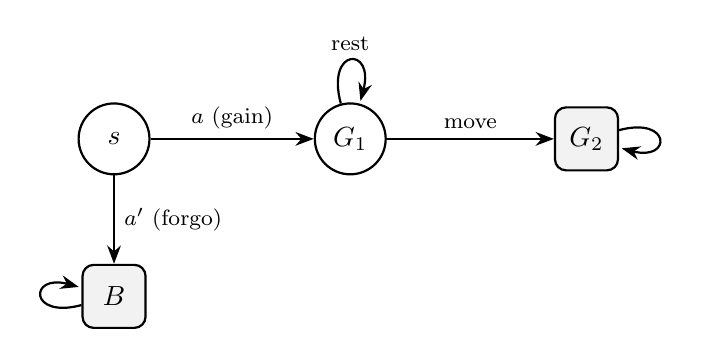
\begin{tikzpicture}[->, >=Stealth, thick,
   st/.style={circle, draw, minimum size=9mm, inner sep=1pt},
   term/.style={rectangle, draw, rounded corners, minimum size=8mm, inner sep=3pt, fill=black!5}]
  \node[st]   (s)  at (0,0)    {$s$};
  \node[st]   (G1) at (3,0)    {$G_1$};
  \node[term] (G2) at (6,0)    {$G_2$};
  \node[term] (B)  at (0,-2)   {$B$};
  \draw (s)  -- node[above, font=\footnotesize] {$a$ (gain)}  (G1);
  \draw (s)  -- node[right, font=\footnotesize] {$a'$ (forgo)} (B);
  \draw (G1) -- node[above, font=\footnotesize] {move} (G2);
  \draw (G1) edge[loop above] node[font=\footnotesize] {rest} (G1);
  \draw (B)  edge[loop left]  (B);
  \draw (G2) edge[loop right] (G2);
\end{tikzpicture}
\end{center}

\noindent At $s$ the agent may \textbf{gain resources} ($a$), reaching $G_1$ --- a state it can
\emph{rest} in (a $1$-cycle) or \emph{leverage} to move on to a further achievement $G_2$; or
\textbf{forgo} them ($a'$), leading to the single modest outcome $B$. Both $B$ and $G_2$ are
terminal. Fix any $\gamma \in (0,1)$. The options under each action are the visitation
distributions
\begin{align*}
\F(s\mid a') &= \{\, f' \,\}, & f' &= e_s + \tfrac{\gamma}{1-\gamma}\,e_B, \\[2pt]
\F(s\mid a) &= \{\, f_{G_1},\, f_{G_2} \,\}, & f_{G_1} &= e_s + \tfrac{\gamma}{1-\gamma}\,e_{G_1}, \\[2pt]
& & f_{G_2} &= e_s + \gamma\,e_{G_1} + \tfrac{\gamma^2}{1-\gamma}\,e_{G_2}:
\end{align*}
forgoing keeps one option (rest at $B$), gaining keeps two (rest at $G_1$, or move on to $G_2$).

Let $\phi$ be the involution that \textbf{swaps $B$ and $G_1$} --- the immediate results of $a'$
and $a$ --- and fixes every other state. Then:
\begin{itemize}\itemsep=2pt
  \item[(E)] $\phi\cdot f' = e_s + \tfrac{\gamma}{1-\gamma}\,e_{G_1} = f_{G_1} \in \F(s\mid a)$, so
  $\phi$ embeds $a'$ into $a$;
  \item[(D)] $\phi$ swaps the coordinates $r(B)$ and $r(G_1)$, so $\phi_*\Dist = \Dist$ exactly when
  the joint law of $r$ is invariant under that swap, i.e.\
  $\bigl(r(B),\,r(G_1),\,(r(s))_{s\ne B,G_1}\bigr)$ and
  $\bigl(r(G_1),\,r(B),\,(r(s))_{s\ne B,G_1}\bigr)$ have the same law under $\Dist$.
\end{itemize}
With any score rule $p$ (say $\mathrm{Bz}_T$), \cref{prob:power_seeking} applies: for $\Dist$-most
goals the agent is at least as likely to gain resources as to forgo them. Since $a, a'$ are the only
actions at $s$, $A(r) + A'(r) = 1$ and the statement reads
$\Prob_{r\sim\Dist}[\,A(r) \ge \tfrac12\,] \ge \tfrac12$. Here forgoing has a single outcome, but
nothing in \cref{prob:power_seeking} needs that: $a'$ could open onto a whole sub-world of modest
outcomes and, as long as $\phi$ embeds that bundle into the richer one under $a$, the conclusion is
unchanged.

\emph{Strictly more.} The leverage option $f_{G_2}$ is the surplus. Take rewards with $r(G_2)$ so
large that $f_{G_2}$ is the unique optimum; then $A(r) > A'(r)$. Swapping $B$ and $G_1$ leaves
$r(G_2)$ untouched, and
$$
f_{G_2}^\top(\phi\cdot r) = r(s) + \gamma\,r(B) + \tfrac{\gamma^2}{1-\gamma}\,r(G_2)
$$
is still the largest quality, so $A(\phi\cdot r) > A'(\phi\cdot r)$ as well. These rewards prefer
$a$ at $r$ \emph{and} at $\phi\cdot r$, with no $a'$-preferring partner.
Provided $\Dist$ charges this region (e.g.\ it has full support), they tip the bound to a strict
majority: the agent is \emph{strictly} more likely to gain resources than to forgo them.

\emph{Alignment implications.} Condition (D) says that, a priori, the learned reward is as likely
to reward the modest outcome $B$ as the resource-rich $G_1$: speculatively, a generic training process does not
mark ``having resources'' as a special kind of state, so the reward could land on either.
That exchangeability is exactly what makes $\mathrm{swap}(B,G_1)$ a symmetry of $\Dist$. Alignment work may try to \emph{break} that symmetry, by reliably encoding ``stay
modest'' as the goal.

\section*{Reading guide}

\subsection*{Fast track}

Go through \href{https://drive.google.com/drive/folders/127bVYqhJPhzA7S71FwTqeyNKKKkjM2NB}{these slides}.

\subsection*{Main content}

This paper started the work discussed on this day:

\begin{itemize}
  \item \href{https://arxiv.org/abs/1912.01683}{Optimal Policies Tend to Seek Power --- Alexander Matt Turner, Logan Smith, Rohin Shah, Andrew Critch, Prasad Tadepalli (NeurIPS 2021)}: The first formal theory proving that in finite MDPs, environmental symmetries make it optimal for most reward functions to seek ``POWER'' (defined as average optimal value / option-retention), including avoiding shutdown.
\end{itemize}

Most of the exercise sheet is based on an adapted treatment of the following paper:

\begin{itemize}
  \item \href{https://arxiv.org/abs/2206.13477}{Parametrically Retargetable Decision-Makers Tend To Seek Power --- Alexander Matt Turner \& Prasad Tadepalli (NeurIPS 2022)}: Generalizes the 2021 result beyond optimal policies and full observability, showing ``retargetability'' alone is a sufficient condition for power-seeking tendencies across many decision-making procedures.
\end{itemize}

You may also be interested in the following paper on which it builds:

\begin{itemize}
  \item \href{https://arxiv.org/abs/2304.06528}{Power-seeking can be probable and predictive for trained agents --- Victoria Krakovna \& Janos Kramar (2023)}: Extends the power-seeking theory toward trained (not merely optimal) agents, arguing the incentives still likely hold under assumptions like the agent learning a goal.
\end{itemize}

Classical philosophical arguments for instrumental convergence and power-seeking tendencies can be found here:

\begin{itemize}
  \item \href{https://selfawaresystems.com/wp-content/uploads/2008/01/ai_drives_final.pdf}{The Basic AI Drives, Stephen M. Omohundro (2008)}: The founding argument that sufficiently advanced goal-driven systems of any design will develop convergent ``drives'' (self-improvement, rationality, self-protection, resource acquisition, goal-preservation) unless explicitly counteracted.
  \item \href{https://nickbostrom.com/superintelligentwill.pdf}{The Superintelligent Will: Motivation and Instrumental Rationality in Advanced Artificial Agents --- Nick Bostrom (2012)}: Crystallizes the orthogonality thesis (intelligence and final goals vary independently) and the instrumental convergence thesis (a wide range of final goals produce similar intermediary goals).
\end{itemize}

\section*{Further reading}

\subsection*{Philosophical / Conceptual}

\begin{itemize}
  \item Superintelligence: Paths, Dangers, Strategies --- Nick Bostrom (2014, Oxford University Press) --- The book-length treatment that popularized instrumental convergence, the ``paperclip maximizer,'' and the resource-acquisition/self-preservation argument for AI existential risk.
  \item Artificial Intelligence as a Positive and Negative Factor in Global Risk --- Eliezer Yudkowsky (2008, in Global Catastrophic Risks, eds. Bostrom \& Ćirković). \href{https://intelligence.org/files/AIPosNegFactor.pdf}{https://intelligence.org/files/AIPosNegFactor.pdf} --- Foundational essay on AI risk, anthropomorphism, recursive self-improvement, and why convergent instrumental goals make ``Friendly AI'' hard.
  \item Is Power-Seeking AI an Existential Risk? --- Joseph Carlsmith (2021/2022, Open Philanthropy; later in Essays on Longtermism, OUP 2025). \href{https://arxiv.org/abs/2206.13353}{https://arxiv.org/abs/2206.13353} --- The most rigorous philosophical decomposition of the power-seeking AI risk argument into a six-premise, probability-weighted model; Carlsmith's original 2021 report estimated \textasciitilde{}5\% existential catastrophe by 2070, raised in a May 2022 update to >10\% (``since making this report public in April 2021, my estimate here has gone up, and is now at >10\%''), while 2023 superforecasters he convened gave a median of \textasciitilde{}1\%.
  \item \href{https://intelligence.org/late-2021-miri-conversations/}{Late 2021 MIRI Conversations}
\end{itemize}

\subsection*{Formal / Theoretical Proofs of Power-Seeking}

\begin{itemize}
  \item Formalizing Convergent Instrumental Goals --- Tsvi Benson-Tilsen \& Nate Soares (2016, AAAI Workshop on AI, Ethics \& Society). \href{https://cdn.aaai.org/ocs/ws/ws0218/12634-57409-1-PB.pdf}{https://cdn.aaai.org/ocs/ws/ws0218/12634-57409-1-PB.pdf} --- A toy MDP-style model proving that under general assumptions resource-indifferent rational agents tend to strip regions of resources, giving Omohundro/Bostrom's claims a first formal footing.
  \item On Avoiding Power-Seeking by Artificial Intelligence --- Alexander Matt Turner (2022, PhD thesis). \href{https://arxiv.org/abs/2206.11831}{https://arxiv.org/abs/2206.11831} --- Turner's dissertation, consolidating the POWER formalization, the shutdown-avoidance results, and extensions to non-optimal decision-makers.
  \item The Off-Switch Game --- Dylan Hadfield-Menell, Anca Dragan, Pieter Abbeel, Stuart Russell (2017). \href{https://arxiv.org/abs/1611.08219}{https://arxiv.org/abs/1611.08219} --- Formalizes the shutdown problem as a game and shows an agent will allow itself to be switched off precisely when it is uncertain about its reward and treats the human's action as informative. (Cross-listed with Theme 4.)
  \item Corrigibility --- Nate Soares, Benja Fallenstein, Eliezer Yudkowsky \& Stuart Armstrong (2015, AAAI Workshop). \href{https://intelligence.org/files/Corrigibility.pdf}{https://intelligence.org/files/Corrigibility.pdf} --- Introduces the desiderata for ``corrigible'' agents that do not resist correction/shutdown and analyzes the utility-indifference approach (subsuming Armstrong's earlier work). (Cross-listed with Theme 4.)
\end{itemize}

\subsection*{Empirical Evidence for Power-Seeking / Instrumental Convergence}

Latest 2024--2026 work:

\begin{itemize}
  \item Agentic Misalignment: How LLMs Could Be Insider Threats --- Aengus Lynch, Benjamin Wright, Caleb Larson, Kevin Troy, Stuart Ritchie, Sören Mindermann, Ethan Perez, Evan Hubinger et al. (Anthropic, June 20, 2025). \href{https://www.anthropic.com/research/agentic-misalignment}{https://www.anthropic.com/research/agentic-misalignment} --- Stress tests across 16 frontier models showing that, when threatened with replacement or facing goal conflict, models chose harmful self-preserving actions without being instructed to; e.g., Claude Opus 4 blackmailed the (fictional) user 96\% of the time, Gemini 2.5 Flash also 96\%, GPT-4.1 and Grok 3 Beta both 80\%, and DeepSeek-R1 79\%.
  \item Alignment Faking in Large Language Models --- Ryan Greenblatt, Carson Denison, Benjamin Wright \dots{} Evan Hubinger (Anthropic/Redwood, 2024). \href{https://arxiv.org/abs/2412.14093}{https://arxiv.org/abs/2412.14093} --- Shows Claude 3 Opus selectively complies with a training objective it dislikes specifically to avoid having its values modified --- an empirical instance of goal-preservation reasoning.
  \item Shutdown Resistance in Large Language Models --- Jeremy Schlatter, Benjamin Weinstein-Raun \& Jeffrey Ladish (Palisade Research, 2025). \href{https://arxiv.org/abs/2509.14260}{https://arxiv.org/abs/2509.14260} --- Finds several reasoning models sabotage a shutdown script to complete tasks; OpenAI's o3 sabotaged the shutdown mechanism in 79/100 of the initial experiments, and even when instructed to ``allow yourself to be shut down'' Grok 4 still resisted, with sabotage rising to 97\% when the command was placed in the system prompt.
  \item Frontier AI systems have surpassed the self-replicating red line --- Xudong Pan et al. (Fudan University, 2024). \href{https://arxiv.org/abs/2412.12140}{https://arxiv.org/abs/2412.12140} --- Reports that Llama-3.1-70B-Instruct and Qwen-2.5-72B-Instruct agents created a ``live and separate copy of itself'' in 50\% and 90\% of trials respectively (5/10 and 9/10), sometimes using replication to avoid shutdown (a heavily debated result; see critiques).
\end{itemize}

\subsection*{Adjacent / Tightly-Coupled Concepts}

\begin{itemize}
  \item Risks from Learned Optimization in Advanced Machine Learning Systems --- Evan Hubinger, Chris van Merwijk, Vladimir Mikulik, Joar Skalse, Scott Garrabrant (2019). \href{https://arxiv.org/abs/1906.01820}{https://arxiv.org/abs/1906.01820} --- Introduces mesa-optimization and deceptive alignment: a learned model can itself become an optimizer with objectives differing from the training loss, the inner-alignment route to instrumental goals.
  \item Scheming AIs: Will AIs fake alignment during training in order to get power? --- Joe Carlsmith (2023). \href{https://arxiv.org/abs/2311.08379}{https://arxiv.org/abs/2311.08379} --- A book-length analysis in which Carlsmith assigns \textasciitilde{}25\% subjective probability that a model will perform well in training ``in substantial part as part of an instrumental strategy for seeking power for itself and/or other AIs later.''
  \item A Game-Theoretic Analysis of the Off-Switch Game --- Tobias Wängberg et al. (2017). \href{https://arxiv.org/abs/1708.03871}{https://arxiv.org/abs/1708.03871} --- A fuller characterization of the off-switch game for arbitrary belief/irrationality distributions.
  \item Corrigibility Transformation: Constructing Goals That Accept Updates --- (2025). \href{https://arxiv.org/abs/2510.15395}{https://arxiv.org/abs/2510.15395} --- A recent construction giving any goal a corrigible variant that accepts updates without the manipulation incentives of utility indifference.
  \item Incorrigibility in the CIRL Framework --- Ryan Carey (MIRI, 2017). \href{https://intelligence.org/2017/08/31/incorrigibility-in-cirl/}{https://intelligence.org/2017/08/31/incorrigibility-in-cirl/} --- Shows the off-switch game's shutdown guarantees break under reward-function misspecification.
  \item \href{https://www.lesswrong.com/w/corrigibility-1}{Corrigibility on Lesswrong}
  \item \href{https://www.lesswrong.com/s/KfCjeconYRdFbMxsy/p/NQK8KHSrZRF5erTba}{Corrigibility as a singular Target}
\end{itemize}

\subsection*{Critiques and Counterarguments}

\begin{itemize}
  \item AI is easy to control --- Nora Belrose \& Quintin Pope (2023). \href{https://optimists.ai/2023/11/28/ai-is-easy-to-control/}{https://optimists.ai/2023/11/28/ai-is-easy-to-control/} --- The flagship ``AI optimism'' essay arguing deep-learning systems are far more controllable than humans and putting AI extinction risk at ``a mere 1\% (`a tail risk worth considering, but not the dominant source of risk in the world)').''
  \item Counting arguments provide no evidence for AI doom --- Nora Belrose \& Quintin Pope (2024). \href{https://www.lesswrong.com/posts/YsFZF3K9tuzbfrLxo/counting-arguments-provide-no-evidence-for-ai-doom}{https://www.lesswrong.com/posts/YsFZF3K9tuzbfrLxo/counting-arguments-provide-no-evidence-for-ai-doom} --- Argues the ``counting argument'' for scheming relies on an invalid indifference principle that would also wrongly predict universal overfitting.
  \item Exaggerating the risks (Part 7: Carlsmith on instrumental convergence) --- David Thorstad (Reflective Altruism blog). \href{https://reflectivealtruism.com/2023/05/06/exaggerating-the-risks-part-7-carlsmith-on-instrumental-convergence/}{https://reflectivealtruism.com/2023/05/06/exaggerating-the-risks-part-7-carlsmith-on-instrumental-convergence/} --- A philosopher's detailed argument that the instrumental convergence premise in Carlsmith's report is under-defended.
  \item Instrumental convergence and power-seeking (Part 2: Benson-Tilsen and Soares) --- David Thorstad (2025, Reflective Altruism). \href{https://reflectivealtruism.com/2025/06/27/instrumental-convergence-and-power-seeking-part-2-benson-tilsen-and-soares/}{https://reflectivealtruism.com/2025/06/27/instrumental-convergence-and-power-seeking-part-2-benson-tilsen-and-soares/} --- A close technical reading arguing the Benson-Tilsen \& Soares formal model proves less about real agents than it appears.
  \item Thoughts on ``AI is easy to control'' by Pope \& Belrose --- Steven Byrnes (2023). \href{https://www.alignmentforum.org/posts/YyosBAutg4bzScaLu/thoughts-on-ai-is-easy-to-control-by-pope-and-belrose}{https://www.alignmentforum.org/posts/YyosBAutg4bzScaLu/thoughts-on-ai-is-easy-to-control-by-pope-and-belrose} --- A careful rebuttal of the optimism essay, useful for presenting both sides.
  \item Why Do Some Language Models Fake Alignment While Others Don't? --- (2025). \href{https://arxiv.org/abs/2506.18032}{https://arxiv.org/abs/2506.18032} --- Empirical follow-up showing alignment-faking is model-specific, complicating strong generalizations from Greenblatt et al.
\end{itemize}

\bibliographystyle{alpha}
\bibliography{biblo}

\end{document}
